In this chapter are analyzed all the requirements related to the system. Each section corresponds to a specific category of requirement. In particular the section \ref{sec:ExternalInterface} explain the requirements and the constraints the system must to respect to achieve the goal imposed by the customer, as the user interface.
\section{External interface requirements}\label{sec:ExternalInterface}
\subsection{User interfaces}
The interface of PowerEnJoy can be both for web application and mobile application. From figure \ref{fig:LogPage} to figure \ref{fig:CarInfoPage} are presented some of the most important pages and screens of PowerEnjoy. In particular in figure \ref{fig:MapPage} is showed the home page of the PowerEnJoy's application, it is composed by a map and some marker located on the map depending of the position of the car. It's important to understand that only the car in a free state are showed within the map. The figure \ref{fig:CarInfoPage} appears whereas when the user clicks on a marker in the map and shows the information of the selected car and a button to reserve it.
	\begin{figure}[H]
		\centering
		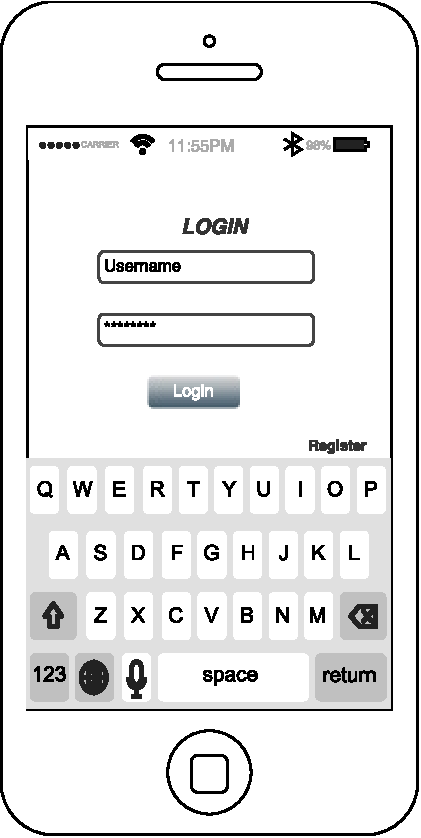
\includegraphics[height=8cm]{Resources/LoginMockup.pdf}
		\caption{Login page}
		 \label{fig:LogPage}
	\end{figure}
	\begin{figure}[H]
		\centering
		\includegraphics[height=8cm]{Resources/RegistrationMockup.png}
		\caption{Registration page}
		 \label{fig:RegistrationPage}
	\end{figure}
	\begin{figure}[H]
		\centering
		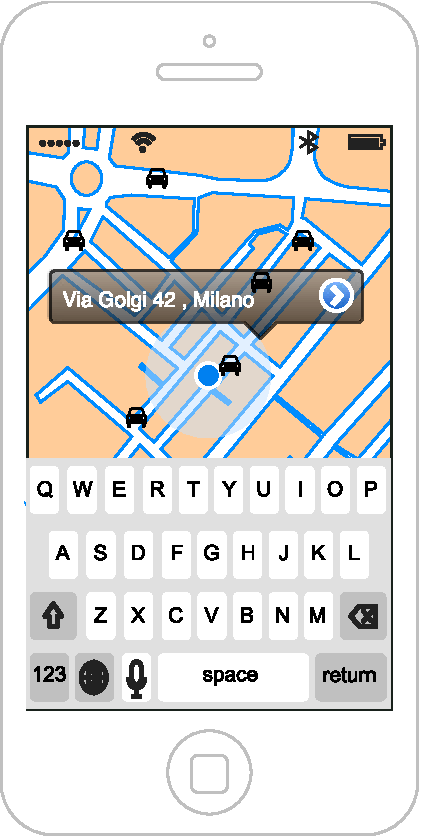
\includegraphics[height=8cm]{Resources/MapMockup.pdf}
		\caption{Home page or Map page}	
		 \label{fig:MapPage}	
	\end{figure}
	\begin{figure}[H]
		\centering
		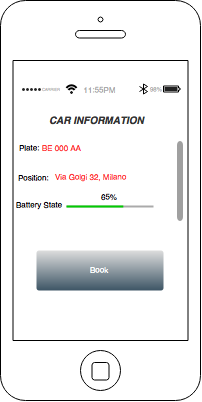
\includegraphics[height=8cm]{Resources/CarInfo.png}
		\caption{Car information page}	
		 \label{fig:CarInfoPage}
	\end{figure}